%Introduction

\section{Heaven}

The architecture of the \textsc{Test Stand} consists in at leas three stand alone modules, \textsc{Streamer}, \textsc{RSP Engine} and \textsc{Result Collector}, that establish a mono-directional communication flow. 
Section \ref{sec:requirements} reports the requirements \name must fulfil and Chapter \ref{chap:heaven} describes how to cover them. In particular, some of this requirements directly affect the implementation experience of \namens , this the case of [R.10] i.e. the need of an \textit{Extendible Design} and [R.11], which states the necessity of an \textit{Event-base architecture} to properly face RSPEngines, which usually exploit this communication pattern.

Developing an \textit{Extendible} \textsc{Test Stand} to handle any RSP Engine requires two abstractions:
\begin{itemize}
\item \textit{Event}
\item \textit{Event Processor}
\end{itemize} 

The \textit{Event} is required to build a hierarchical communication. \textsc{Test Stand} handle many events flows, a lest three: one for the RSP Engine module, one for the communication between modules and one to communicate with the user. Next section about data clarify how the communication is structured and it explains how the components communicates. The \textit{Event Processor} guarantees the system to be modular, it simplifies the behaviour of each component of the \textsc{Test Stand} structure, standardizing the interaction. 

Thus, to define what is a module we can say: a module is an \textit{Event Processor} which can be positioned everywhere in the pipeline which represent the \textsc{Test Stand} architecture.  As a matter of facts, specific implementations of a module may reduce the generality of this definition and also the flexibility of the module itself. themselves.	

Last but not least the the requirement [R.4] states the \textsc{Test Stand}\textit{ must not be running when the RSP Engine is under execution} (see Section \ref{sec:requirements}. Each module in the system can be seen as a Finite State Machine (FSM). A module can work only if its current state allow processing. An Error State prevents the propagation on errors in the data. The following schema represent the FSM for all the modules of \name, even the Baselines, and also for its external structure, which exploit this behaviour to control execution an stop its process while the RSPEngine is running (see Section \ref{sec:teststand}).

\begin{figure}[tbh]
  \centering
	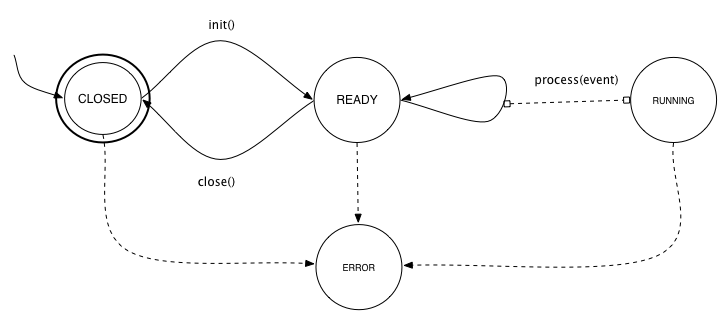
\includegraphics[width=\linewidth]{images/fsm-schema}
	\caption{Module Finite State Machine Automata} 
  	\label{fig:module-fsm}
\end{figure}

Figure \ref{fig:module-fsm} shows the FSA for the module execution. Two methods move form the CLOSED state into the READY one. We state that each module is an EventProcessor, the process() method brings the caller module to the RUNNING state until the execution process ends. The ERROR state may be reached from any point of the execution and the error will be reported to the user.

\section{Events and Data}\label{sec:data-impl}

Chapter \ref{chap:problem-settings} poses the requirements of an Event-based architecture [R.11] for the \textsc{Test Stand} to properly handle the interaction with RSP Engines, which are event-base systems. Moreover, Chapter \ref{chap:heaven} describes \name workflow and how it exchanges events during the execution. The \textsc{Test Stand} modules interact trough events which contains data at different points of the experiment process. \name handles in general three kind of events:

\begin{figure}[tbh]
  \centering
	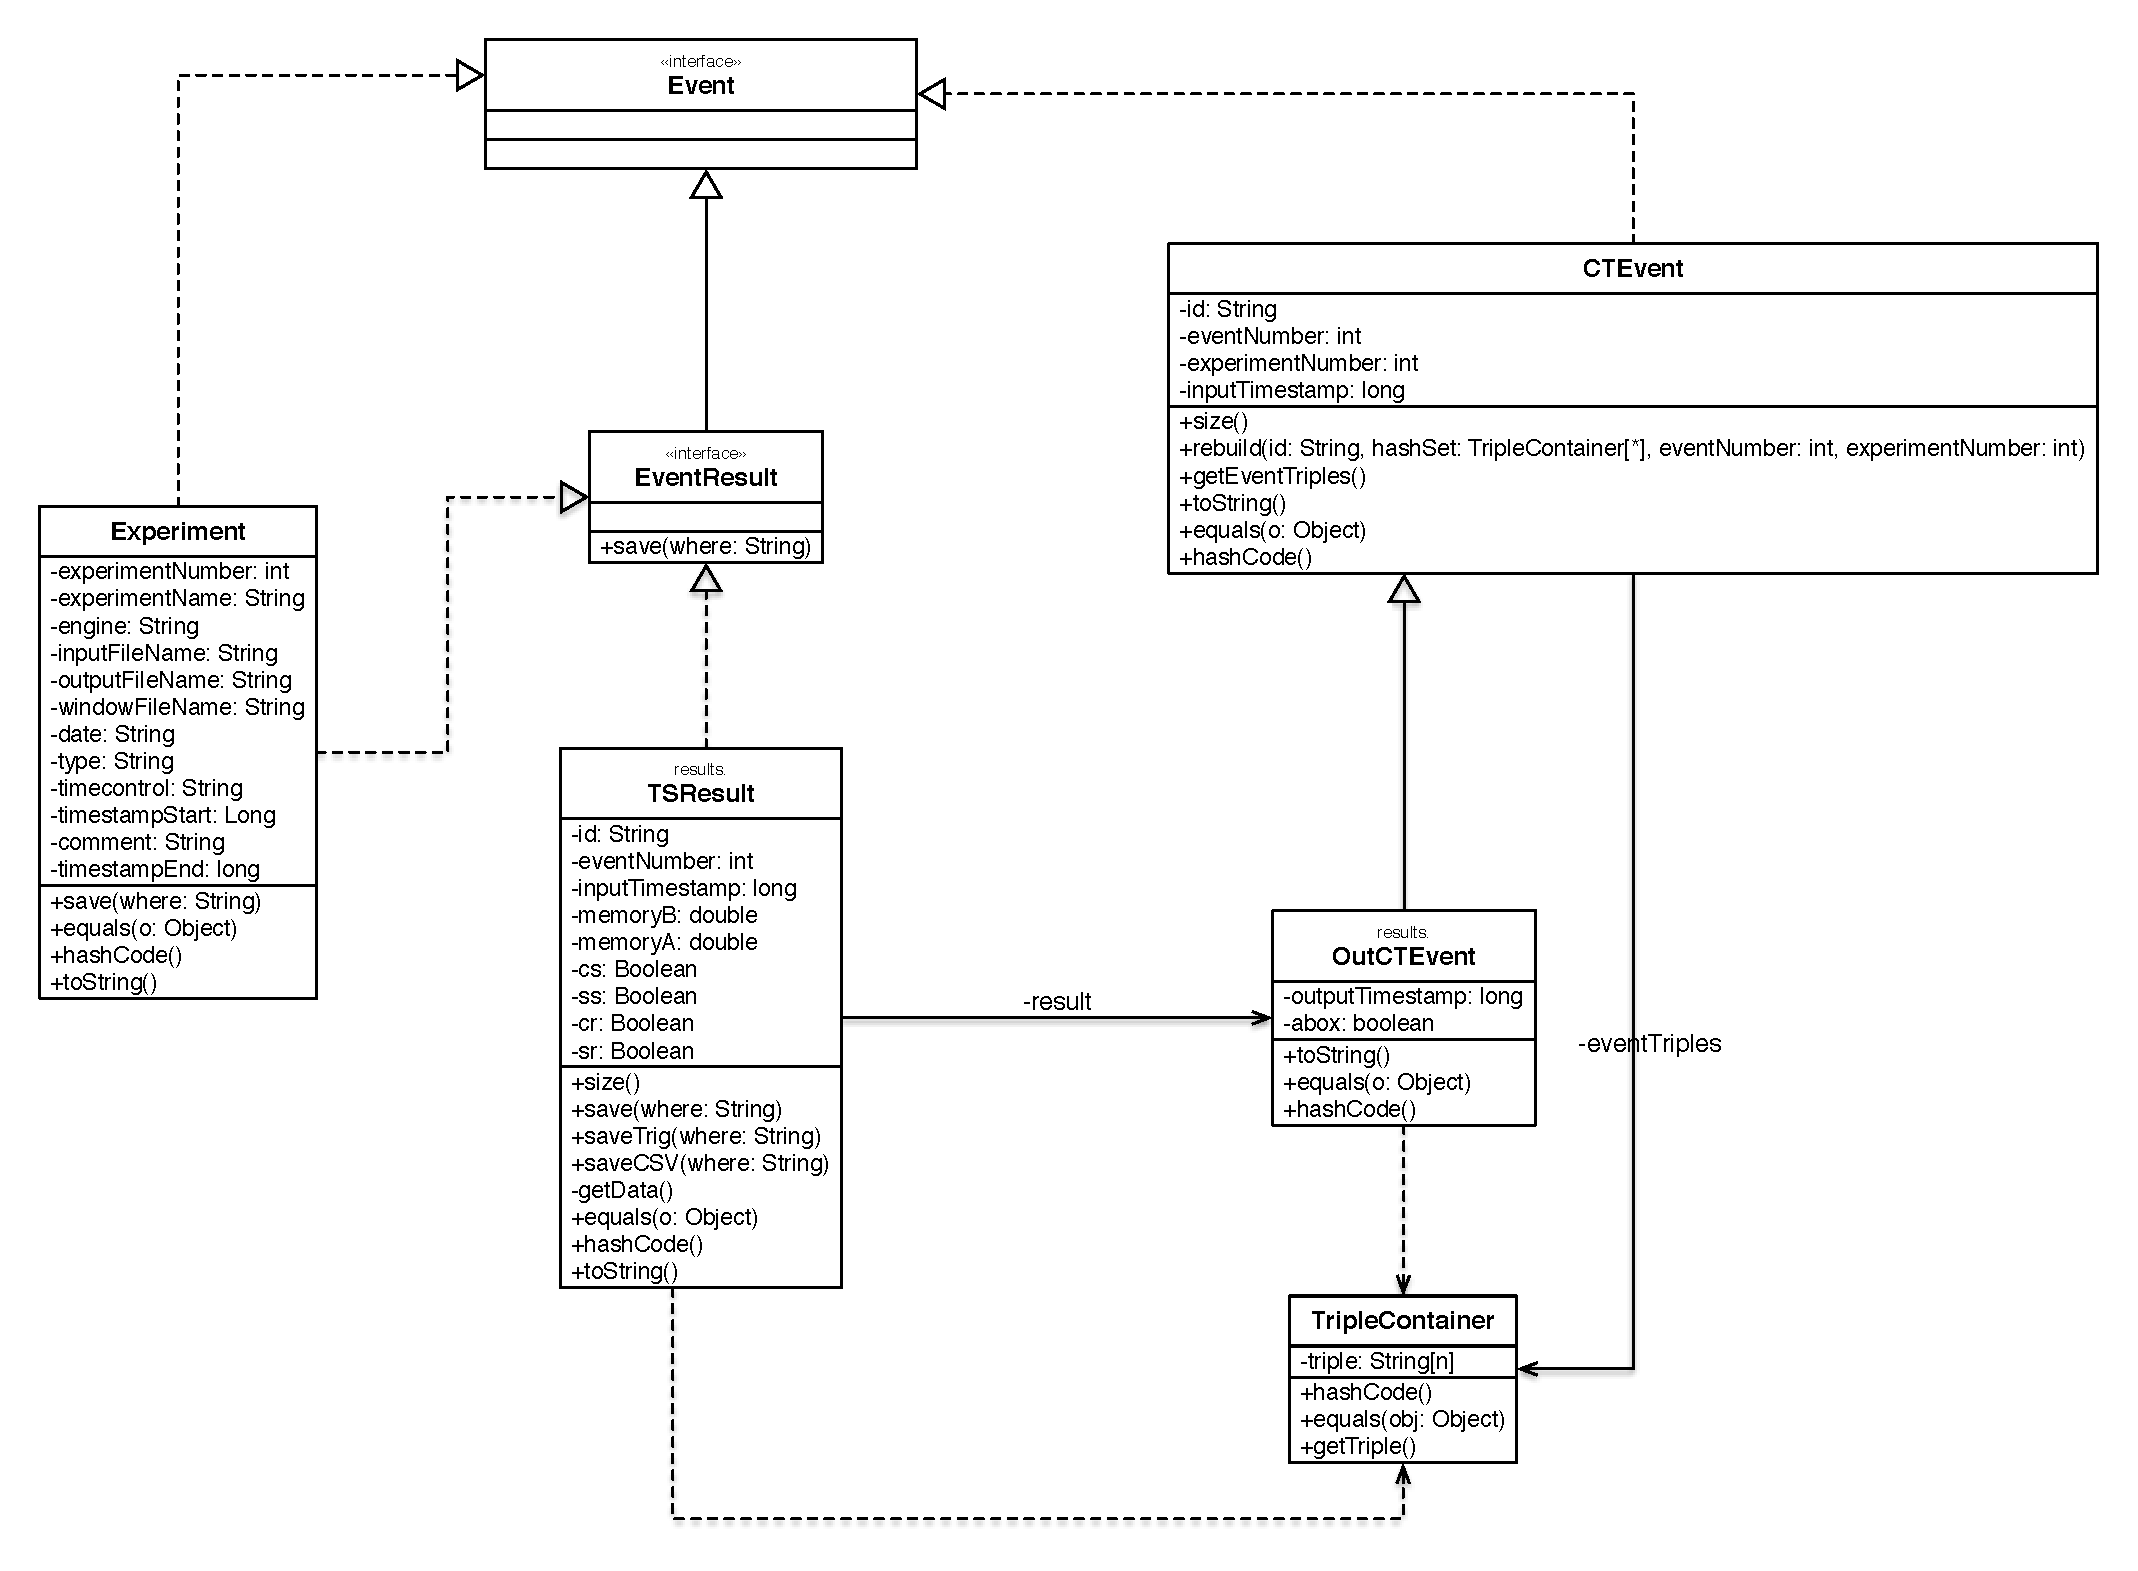
\includegraphics[width=\linewidth]{images/uml_events}
	\caption{UML Schema for all the events involved in the system} 
  	\label{fig:uml_events}
\end{figure}

\begin{itemize}
\item \textit{Experiment} - it represents the tuple $<\mathcal{E}, \mathcal{D},\mathcal{T},\mathcal{Q}>$ and all the experiment metadata like start time or end time.
\item \textit{CTEvent and OutCTEvent} - they contains a set of triples which has the same timestamp. The \textit{OutCTEvent} represents the event produced by the RSPEngine after processing the active window. Figure \ref{fig:uml_events} show the inheritance relation between \textit{CTEvent} and \textit{OutCTEvent}
\item \textit{TSResult} - it wraps the \textit{OutCTEvent} adding the information about the minimal sensor data: memory and latency and complete and soundness if it evaluated at runtime (see Section \ref{sec:requirements})
\end{itemize}

\name requires an initialization phase to prepare the \textit{Experiment} and pass it to the \textsc{Test Stand} . The current implementation we exploits a property file which all the concrete information about Experiment: ID and the tuple $<\mathcal{E}, \mathcal{D},\mathcal{T},\mathcal{Q}>$. 
The \textit{CTEvent} and the \textit{OutCTEvent} classes carry RDF triples in NT-Triple\footnote{http://www.w3.org/2001/sw/RDFCore/ntriples/}, which is the easiest RDF serialisation to parse. This serialisation was chose to fulfil requirement [R.12], which demands an \textit{Easy-to-Parse RDF Serialisation for the events presented to the RSP Engine in exam}. Figure \ref{fig:uml_events} shous also that the RDF Triples are stored in the events into the \textit{TripleContainer} wrapper,in order to redefine the triple hashcode and equals method guaranteeing their uniqueness of the triple for each \textit{CTEvent} or \textit{OutCTEvent}.

\section{Modules}

\subsection{Streamer}	\label{sec:streamer-impl}
\begin{figure}[tbh]
  \centering
	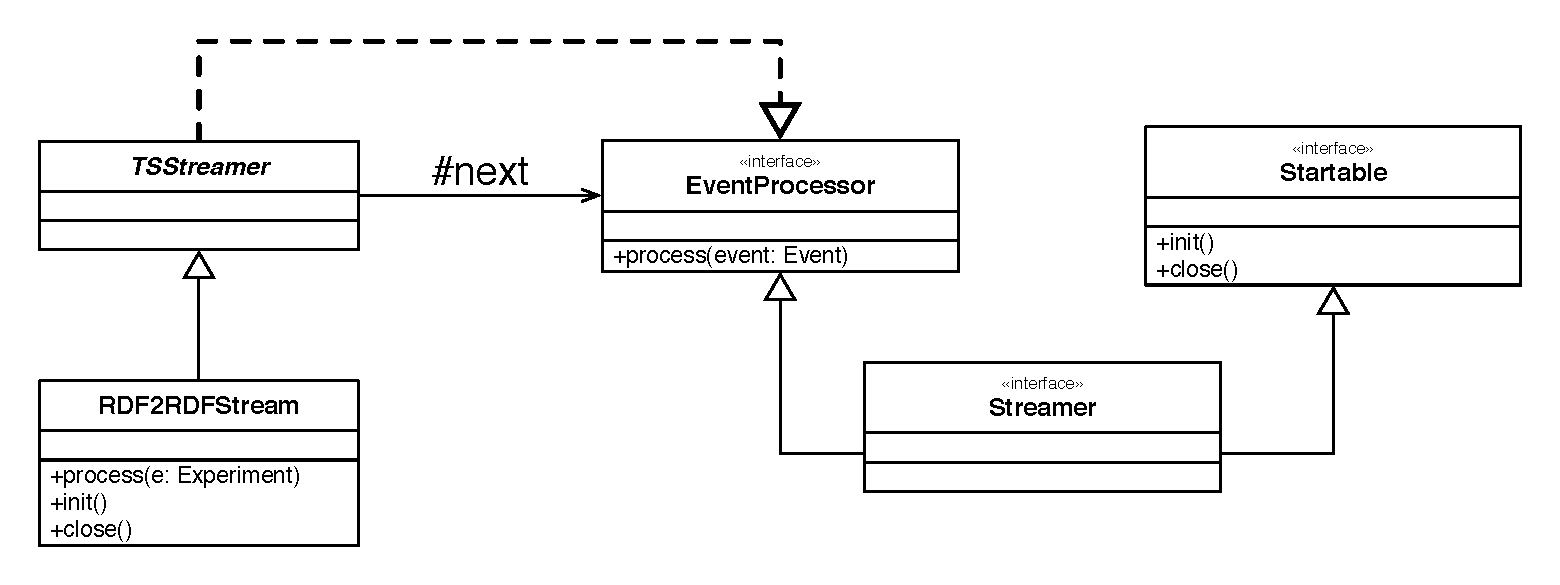
\includegraphics[width=\linewidth]{images/uml_tstreamer}
	\caption{Streamer UML Schema with TSStreamer and Implementation example} 
  	\label{fig:uml_tstreamer}
\end{figure}

The head-module in the \textsc{Test Stand} pipeline is the on \textit{TSStreamer}, which is the most general implementation of the \textsc{Streamer} as Figure \ref{fig:uml_tstreamer} shows. The \textit{TSStreamer} processes an \textit{Experiment} and communicates with one Event Processor , which instead process \textit{CTEvent} and follows in the pipeline. How the \textit{TSStreamer} communicates with the following \textit{EventProcessor} may changes to follow the user needs. The actual implementation , the RDF2RDFStream, was developed to sustain experiments as they are presented in Chapter \ref{chap:evaluation}
It is worth to note that we use LUBM Benchmarks to generate the data for the experiments. For this reason, the RDF2RDFStream module builds an RDFStream starting from the static data produced by LUBM.

\begin{figure}[tbh]
  \centering
	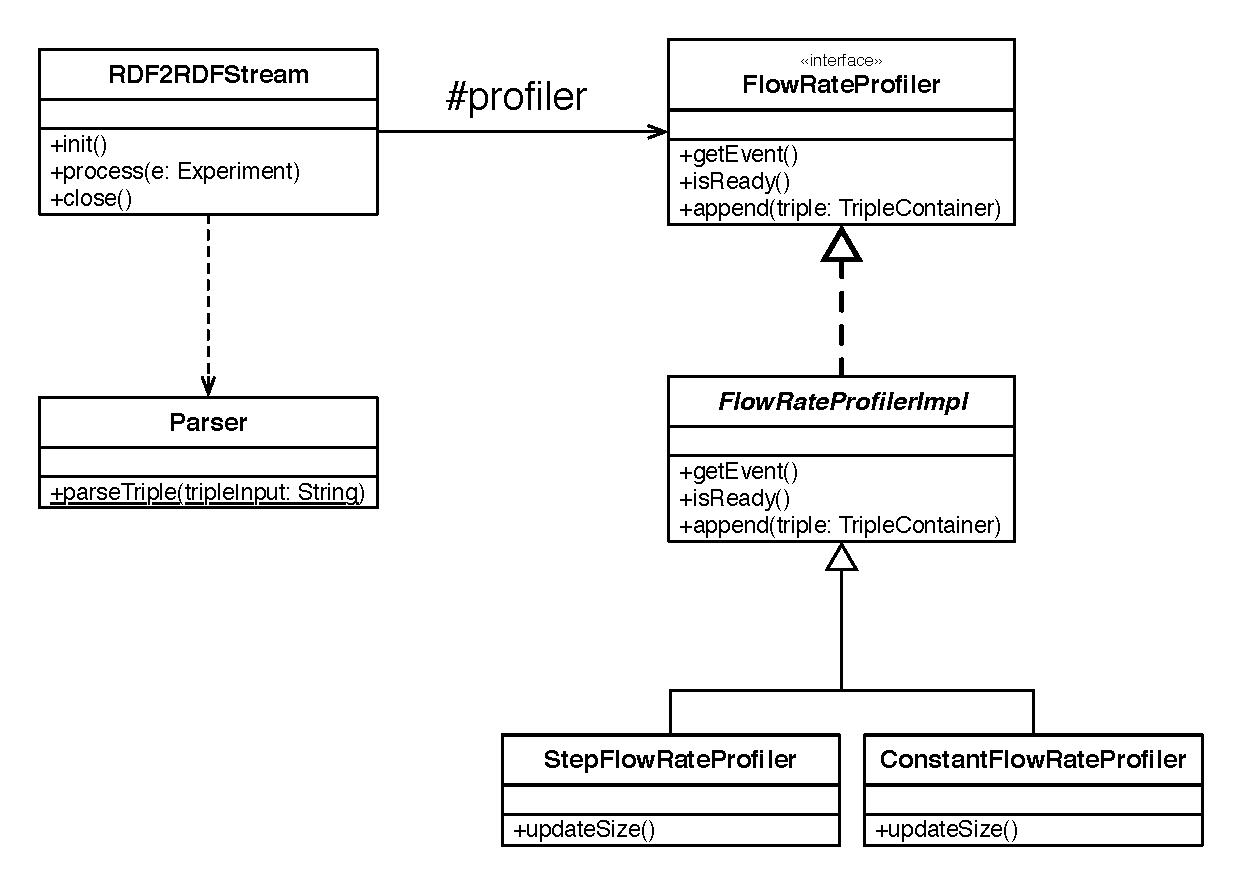
\includegraphics[width=0.75\linewidth]{images/uml_flowrateprofiler}
	\caption{RDF2RDFStream internal UML Schema} 
  	\label{fig:uml_flowrateprofiler}
\end{figure}


Figure \ref{fig:uml_flowrateprofiler} shows how the \textit{RDF2RDFStream} exploits two components: a statically accessed\textit{Parser} and the \textit{FlowRateProfiler}. 

The \textit{Parser} reads in memory one by one the triples in the file, guaranteeing data independence [R.1] and do not influencing the memory footprint [R.5] by allocating only the memory necessary to parse a triple. The file is generated by LUBM(1000,0), which means 1000 different universities with random generation seed 0. 
The \textit{FlowRateProfiler} determines the number of triples to add to a \textit{CTEvent} and builds such an event. In this way, \textit{RDF2RDFStream} can generate different RDF streams $\mathcal{D}$, which differentiate on the number of contemporary triples in the stream. The \textit{FlowRateProfiler} builds the triple according with a function $y=f(x)$ where $x$ is the number of the \textit{CTEvent} and the $y$ is the number of this \textit{CTEvent} will contain. Practically $f$ can be any function from N to N. We develop two \textit{FlowRateProfiler} for our experiment: 
\begin{itemize}
\item \textit{ConstantFlowRateProfiler}, which maintains the same number of triples for each events over all the experiment  
\item \textit{StepFlowRateProfile}, which has a constant number of triple for max $x$ \textit{CTEvents}, then suddenly changes the number of triple $y$.
\end{itemize}
Other implementations are available in \name right now, but are not used in the experiments:
\begin{itemize}
\item \textit{LinearStepFlowRateProfile}, which stream $x$ CTEvents of dimension $y$, in terms of triples, then linearly increase the number of a quantity $n$.
\item \textit{ConstantRandomFlowRateProfiler}, which changes $y$ and $x$ according with two random generators directed by two seeds.
\end{itemize}

\subsection{Result Collector} 

\noindent The \textsc{ResultCollector} is the acquisition system that collects the query results and the measurements data gathered by the \textsc{Test Stand} during the execution.

\begin{figure}[tbh]
  \centering
	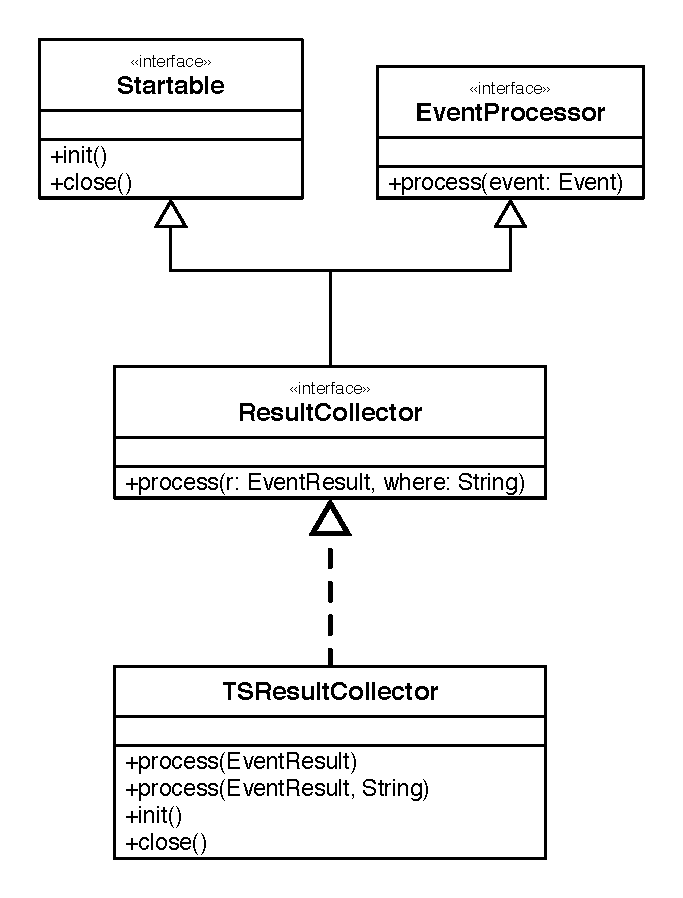
\includegraphics[width=\linewidth]{images/uml_resultcollector}
	\caption{ResultCollector UML Schema with events Experiment, TSResult and OutCTEvent} 
  	\label{fig:uml_resultcollector}
\end{figure}

The UML Schema in Figure \ref{fig:uml_resultcollector} shows the standard implementation, named \textit{TSResultCollector}, whcih implements the \textit{ResultCollector} interface, a proxy for the \textit{EventProcessor}. The \textit{TSResultCollector} stays at the end position in the pipeline which compose the \textsc{Test Stand}. It is responsible of saving data  in a way that does not care about the data format, because of the requirement [R.7], which demands to \textit{enable users extensions with new software sensors and specific measurements collection}. The \textbf{Active Event Pattern} consists into an interface, \textit{EventResult}, which exposes methods that hides the procedure, leaving to the provider of the event the responsibility to implement the method, according with his needs. Figure \ref{fig:uml_resultcollector} shows the relation between the  \textit{EventResult}, interface and the \textit{TSResultCollector}, which calls this method over all the events passed to it during the execution. 


\begin{figure}[tbh]
  \centering
	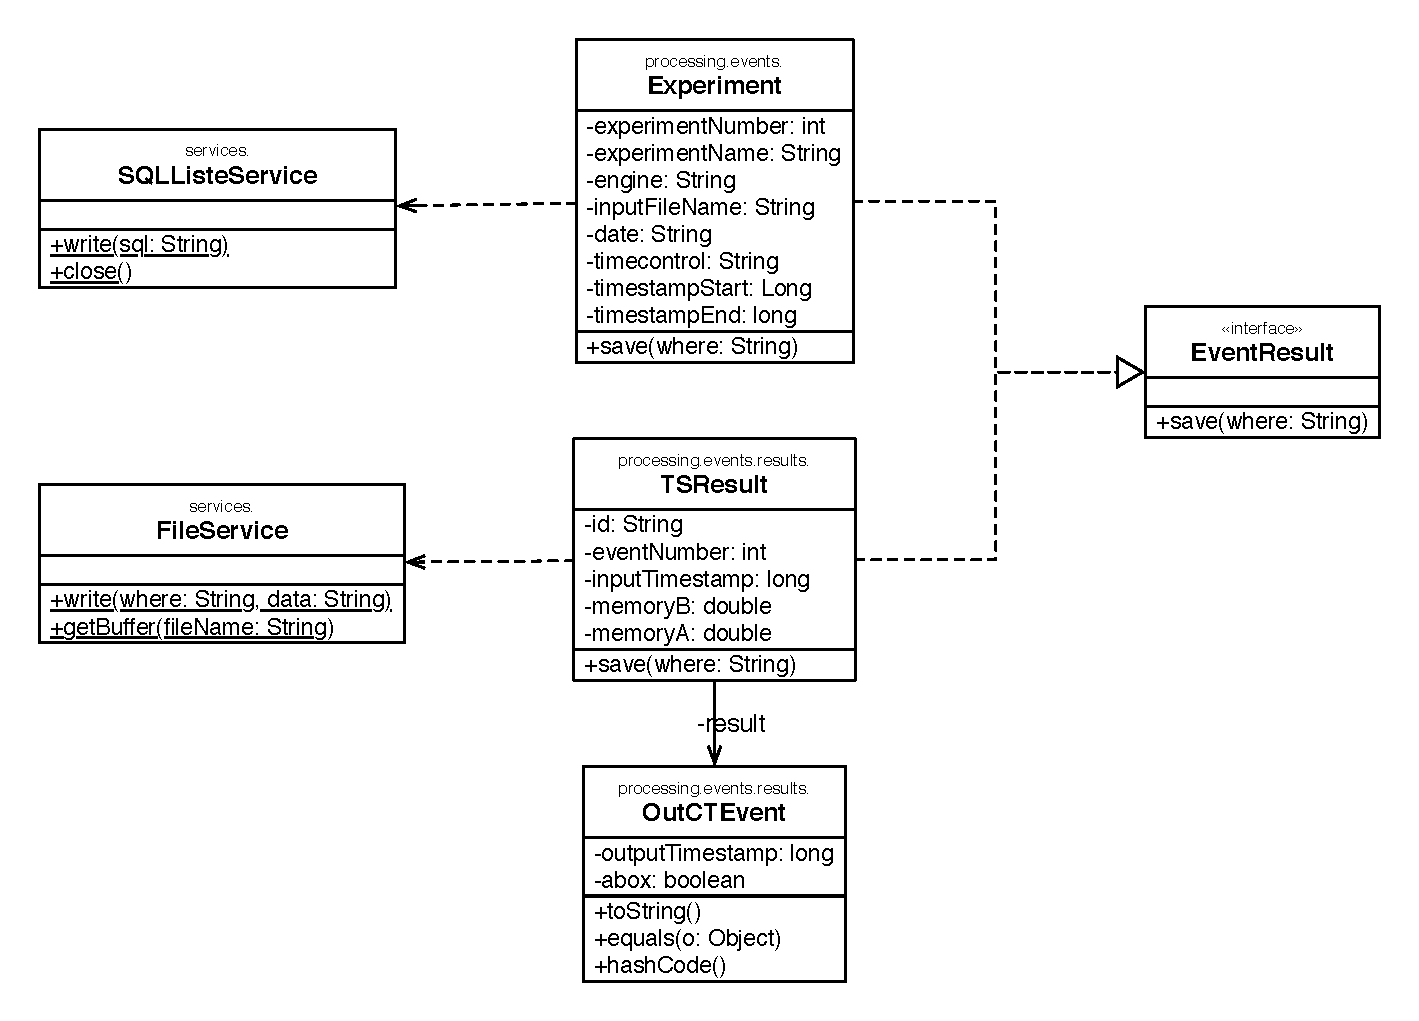
\includegraphics[width=\linewidth]{images/uml_resultcollector_events}
	\caption{ResultCollector events  UML Schema: Experiment, TSResult and OutCTEvent} 
  	\label{fig:uml_resultcollector_events}
\end{figure}

Moreover, Figure \ref{fig:uml_resultcollector_events}, shows how different events in the system exploit the \textit{EventResult} interface. In the current implementation the \textit{TSResultCollector} handles two kinds of event:
\begin{itemize}
\item \textit{TSResult} - it saves the data of the query results into a TriG\footnote{http://www.w3.org/TR/trig/} file where the graph key is the event id inside the experiment, while it save the sensor data with event id into a CSV\footnote{$http://en.wikipedia.org/wiki/Comma-separated_values$} file. 
\item \textit{Experiment}. It saves the experiment metadata and the tuple \\ $<\mathcal{E},\mathcal{D},\mathcal{T},\mathcal{Q}>$ as description field into SQLite\footnote{https://sqlite.org/} database.
\end{itemize} 

The two saving procedure exploits service classes, the \textit{SQLLIsteService} and the \textit{FileService} in Figure \ref{fig:uml_resultcollector_events}, which exposes statical methods to interact with the file-system. The goal is to reduce the system complexity and offer a single point to interact with the file-system, which usually is a slow operation, to avoid parallel interactions that may influence the experiment. 


\subsection{Test Stand Supporting Structure}\label{sec:teststand}


\begin{figure}[tbh]
  \centering
	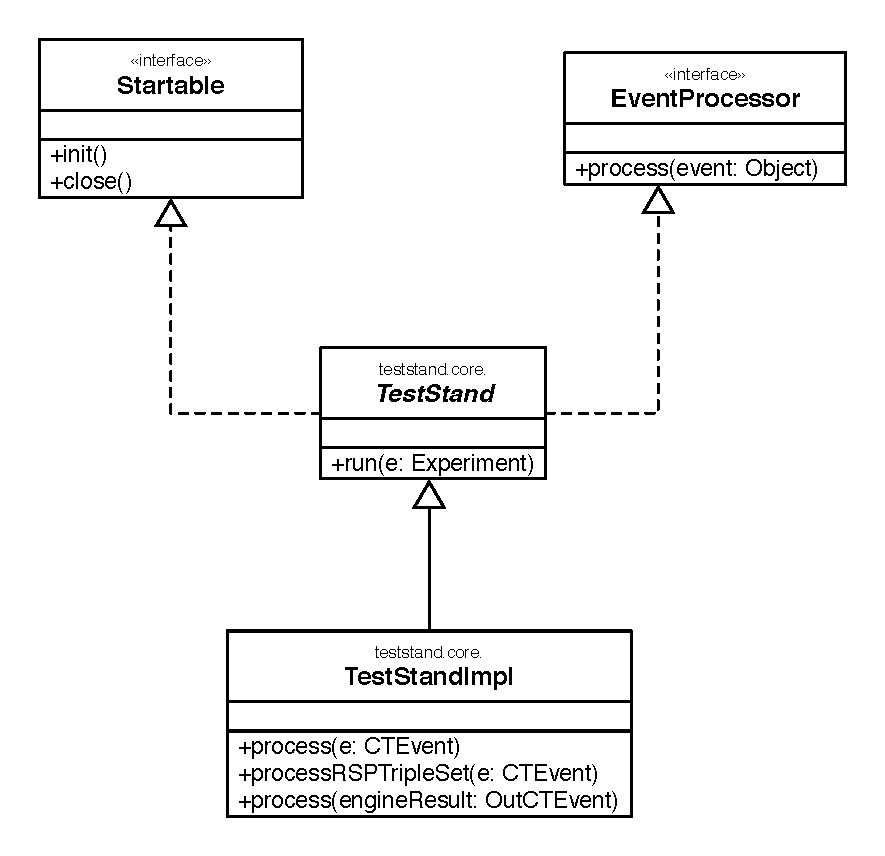
\includegraphics[width=\linewidth]{images/uml_teststand}
	\caption{UML Schema the TestStand} 
  	\label{fig:uml_teststand}
\end{figure}


\name \textsc{Test Stand} was defined as set of modules which interact exchanging events during the execution. However, Chapter \ref{chap:havean} describes at the design level the presence of an external structure which orchestrates the communication between the \textsc{Streamer} the \textsc{RSP Engine} and the \textsc{ResultCollector}. This external structure and its implementation allow the modules to communicate and exposes the APIs for users interaction. Figure \ref{fig:uml_teststand} shows both these classes called \textit{TestStand} and its current implementation is the \textit{TestStandImpl}.


Figure \ref{fig:uml_teststand} shows that the \textit{TestStand} structure is and \textit{EventProcessor} as other modules. Figure \ref{fig:uml_teststand_modules} shows how  modules are referenced by the \textit{TestStand} class. The \textit{TSStreamer}, the \textit{RSPEngine} and the \textit{TSResulCollector} are passed to the \textit{TestStandImpl} trough an initialisation class which receives the configuration file, and set this modules up according with the requirements [R.1] for data independence  [ R.2 and R.3] for engine independence and query independence. Once the set-up phase is complete the \textit{TestStandImpl} is initialized, and it consequently initialises all the upstanding modules. The \textit{Experiment} is created externally and passed to the \textit{TestStandImpl} to start the execution. 

\begin{figure}[tbh]
  \centering
	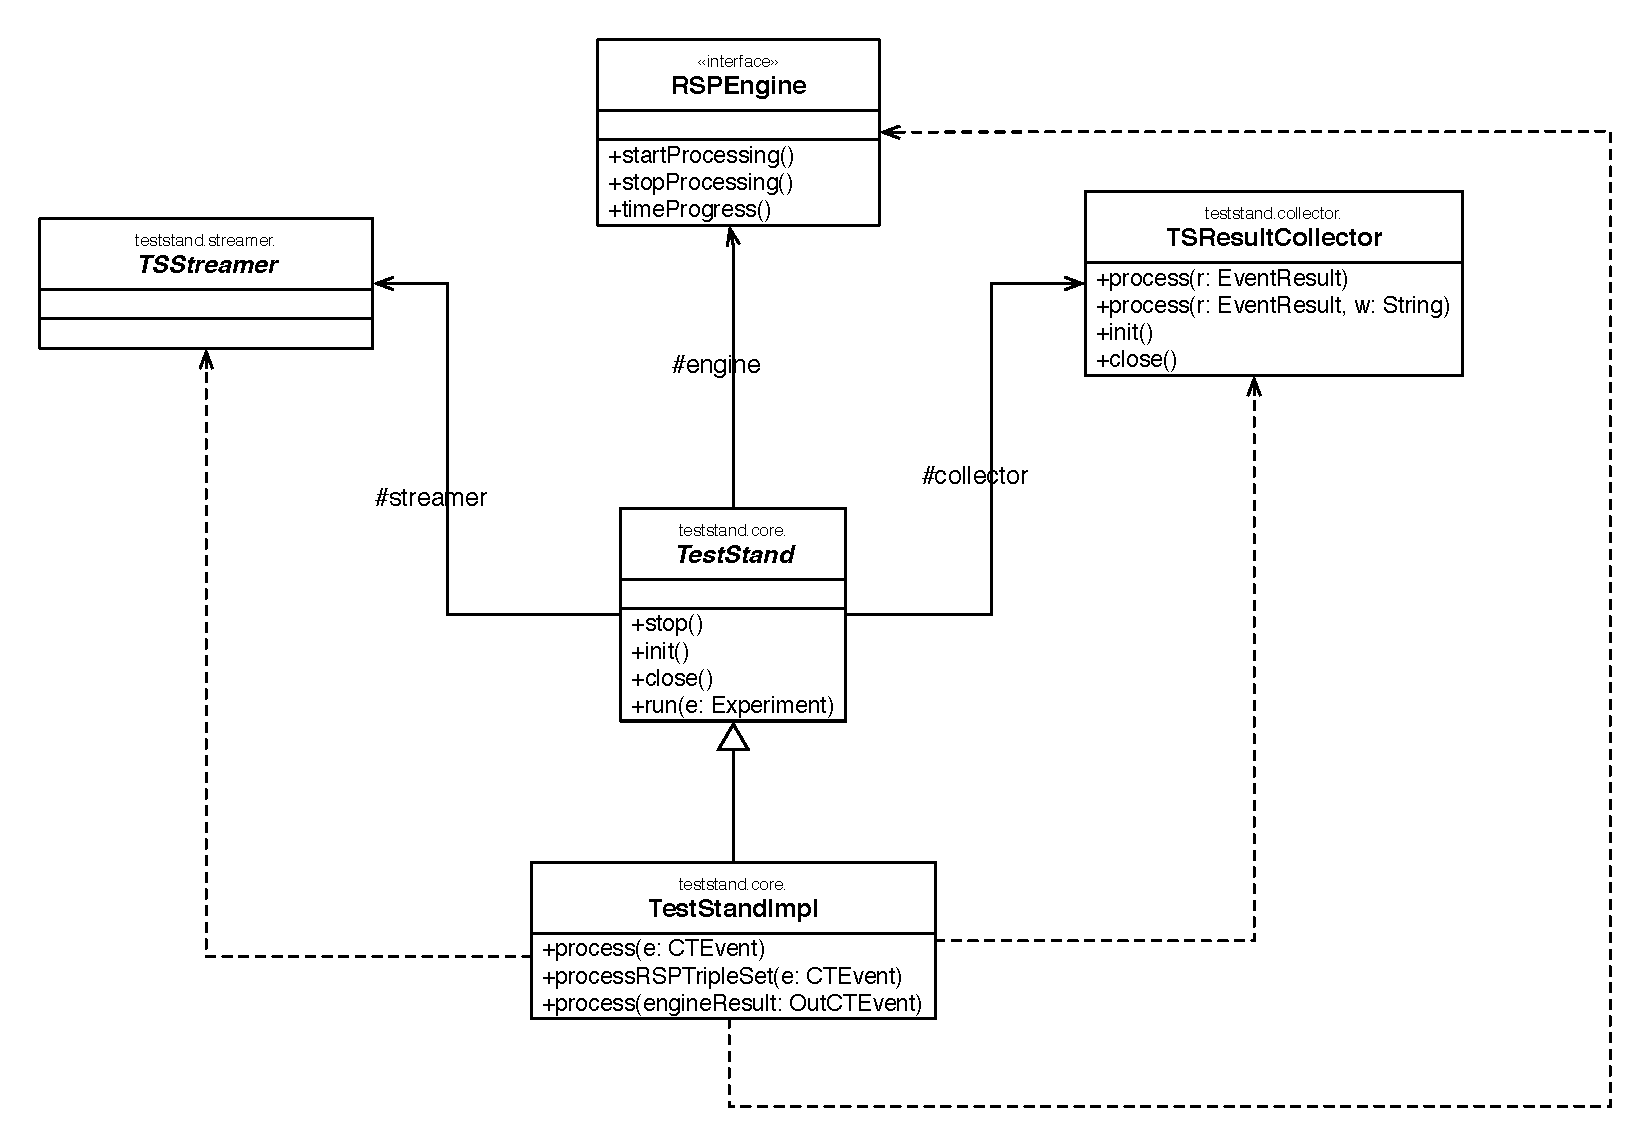
\includegraphics[width=0.90\linewidth]{images/uml_teststand_modules}
	\caption{UML Schema the TestStand with the upstanding modules: TSStreamer, RSPEngine, TSResultCollector} 
  	\label{fig:uml_teststand_modules}
\end{figure}

During the execution \textit{TestStandImpl} intercepts the \textit{CTEvents} form the \textit{TSStreamer} and send them to to the \textit{RSPEngine} as described in Section \ref{sec:arch-workflow}. According with the \textit{Experiment} specification the \textit{TestStandImpl} turn off or on its sensors. It calculates latency starting a timer when the \textit{CTEvent} arrives and stopping the timer when it \textit{RSPEngine} outputs the results. It calculates memory in asking to the JVM in both the point above [R.6]. To fulfil requirements [R.7] any new measurement can be positioned between this two phases of interaction, when the \textit{RSPEngine} is not running yet or when it has finished the computation. Once the \textit{OutCTEvents} comes form the \textit{RSPEngine}, the \textit{TestStandImpl} receives it and wraps it within a \textit{TSResult}, then it sends the query results data together with the measures to the \textit{TSResultCollector} fulfilling [R.8] and supporting [R.9] for further analysis with the Analyser.
%
%R.6 include basic set of performance measurements [?].
%R.7 enable users extensions with new software sensors and specific measure-
%ments collection.
%R.8 support performance measurements collection for further analysis.

\section{Baselines}\label{sec:baselines-impl}

\name Baselines are four elementary implementation of an RSP Engine which follow the design proposal presented in Section \ref{sec:baselines}, covering [R.13]. They pipeline Esper\footnote{$http://www.espertech.com/esper/$}, a mature commercial DSMS, with the Jena general purpose rule engine\footnote{http://jena.apache.org/documentation/inference/\#rules
}, a flexible reasoning engine. The motivations behind the choice of Esper and Jena regards the intention to fulfil requirement [R.14], baselines Eligibility, coupling this two good solution for reasoning and CEP, to obtain a fair solution the SR context. 

\begin{figure}[tbh]
  \centering
	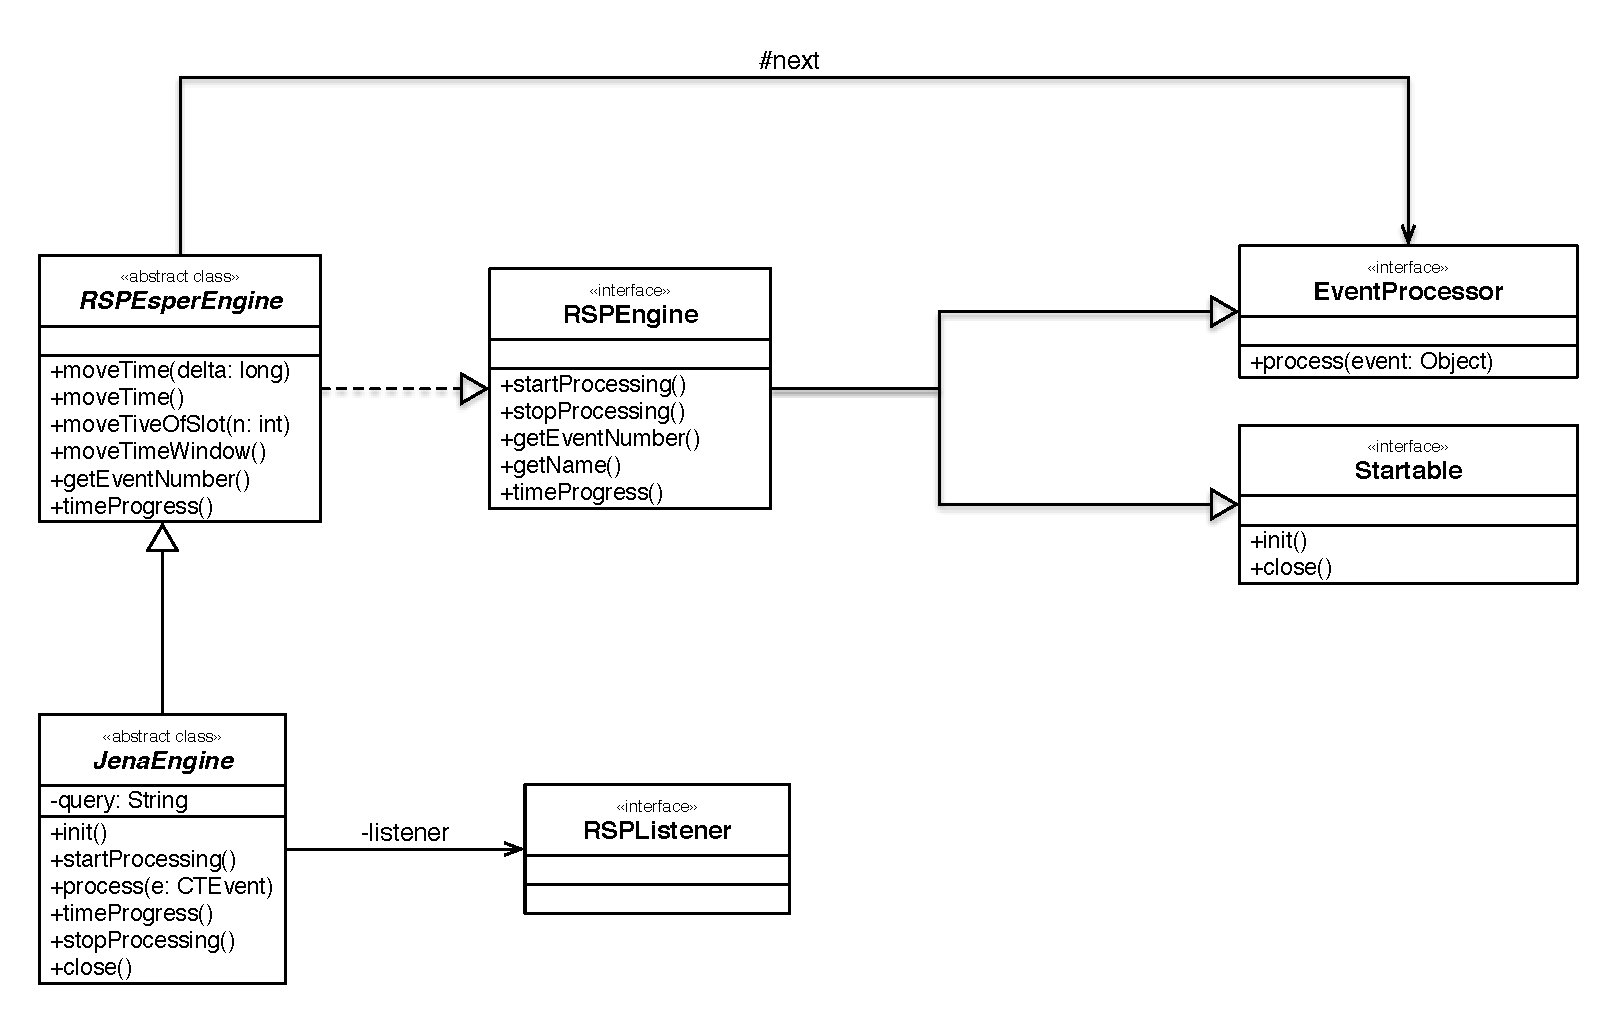
\includegraphics[width=\linewidth]{images/uml_baselines_general}
	\caption{RSPEsper Engine General UML Schema} 
  	\label{fig:uml_baselines_general}
\end{figure}

Figure \ref{fig:uml_baselines_general} shows the general implementation of the baselines: they  exploit the \textit{RSPEngine} interface, a proxy for an \textit{EventProcessor}, implementing the interface into the \textit{RSPEsperEngine} abstract class that includes the esper runtime.  The proposed baselines take advantage of the ability of esper to be temporally controlled by an external agent\footnote{\url{http://esper.sourceforge.net/esper-0.7.5/doc/reference/en/html_single/index.html#api-controlling-time}} by sending time-keeping events to synchronise the internal time flow. One time-keeping event is sent before injecting the triples within a \textsc{CTEvent} and another one after all triples in \textsc{CTEvent} were sent. In this way all the triples in the \textsc{CTEvent} are consider contemporary by the baselines. To enable external time control the RSPEngine interface exposes the moveTime() method, whose implementation depends on the particular RSP Engine in use. The next attributes, represents the general \textit{EventProcessor} which follows the RSPEngine in the \textsc{Test Stand} pipeline, it can be any modules which processes \textit{CTEvent}.

\begin{figure}[tbh]
  \centering
	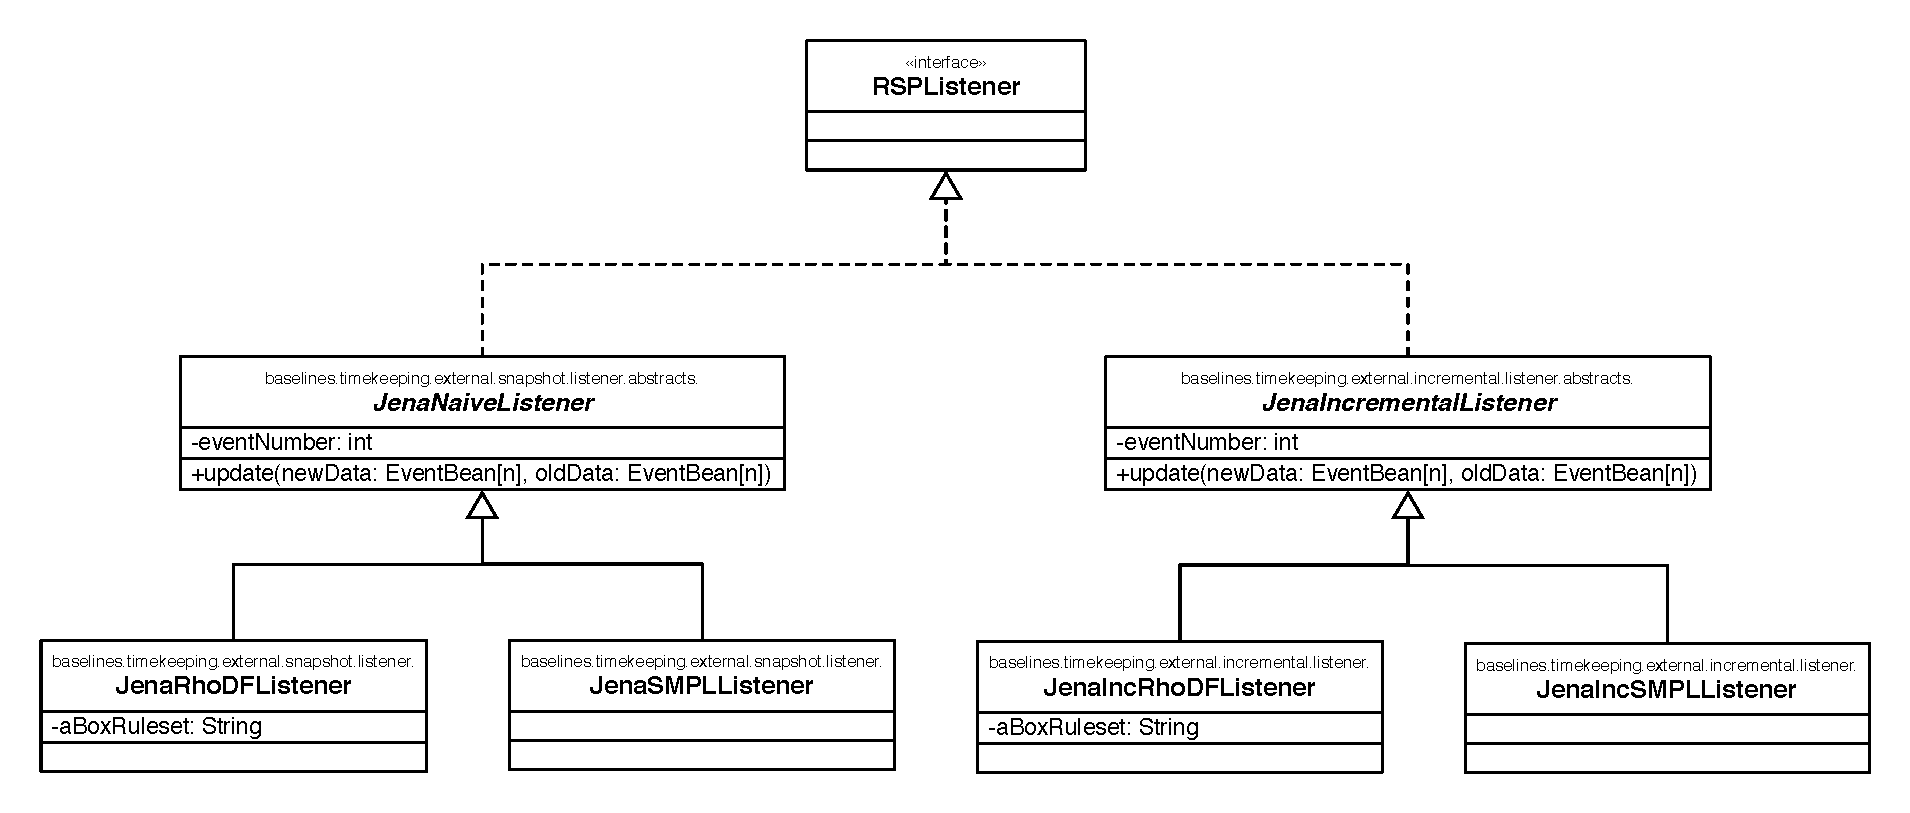
\includegraphics[width=\linewidth]{images/uml_baselines_listener}
	\caption{RSPListener UML Schema} 
  	\label{fig:uml_baselines_listener}
\end{figure}

In Figure \ref{fig:uml_baselines_general} is visible also the interaction between  the RSP Engine, represented by \textit{JenaEngine} abstract class, with the incoming \textit{CTEvent}. The engine is referencing the \textit{RSPListener} responsible to pipeline the Jena rule engine to the DSMS. 

\begin{figure}[tbh]
  \centering
	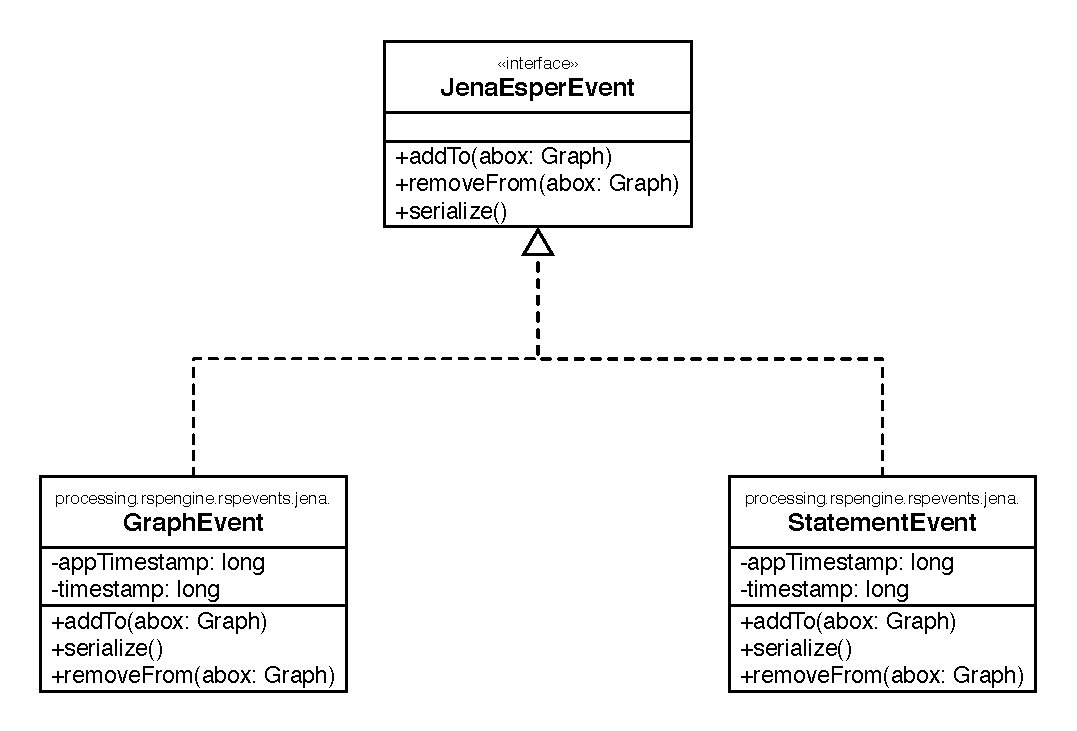
\includegraphics[width=0.5\linewidth]{images/uml_baselines_events}
	\caption{Esper-level events UML Schema} 
  	\label{fig:uml_baselines_events}
\end{figure}

Figure \ref{fig:uml_baselines_listener} shows the different implementations of the \textit{RSPListener}, which specify the reasoning approaches, Naive or Incremental as demanded by [R.15] (baseline relevance), according with the baseline design presented in Section \ref{sec:baselines}. Neither the \textit{JenaNaiveListener} or the \textit{JenaIncrementalListener} specify the entailment regime, which must be defined with specific implementations as it is visible in the Figure.\\

\pagebreak

When a \textit{CTEvents} comes to the RSP Engine it will be transformed into the events handled by the DSMS, \ref{fig:uml_baselines_events}, this translation process influence the latency calculus. Once the processing is complete, the output of the RSP Engine is injected into an \textit{OUTCTEvent} and passed to the next \textit{EventProcessor} in the pipeline, which is the \textsc{Test Stand}. \textit{JenaEsperEvent} interface, as reported in Figure \ref{fig:uml_baselines_events} exposes methods to interact with the RDF model, independently from the event implementation. The figure shows the current two implementation, Graph Based or Triple Based, which cover again [R.15] about baseline Relevance. Moreover, Figure \ref{fig:uml_baselines_rel_listener_event} shows how the \textit{JenaNaiveListener} and the  \textit{JenaIncrementalListener} handles the events which come form the DSMS trough the \textit{JenaEsperEvent} interface, for the case of Graph-based event representation (see Section \ref{sec:baselines} for event details). 

\begin{figure}[tbh]
  \centering
	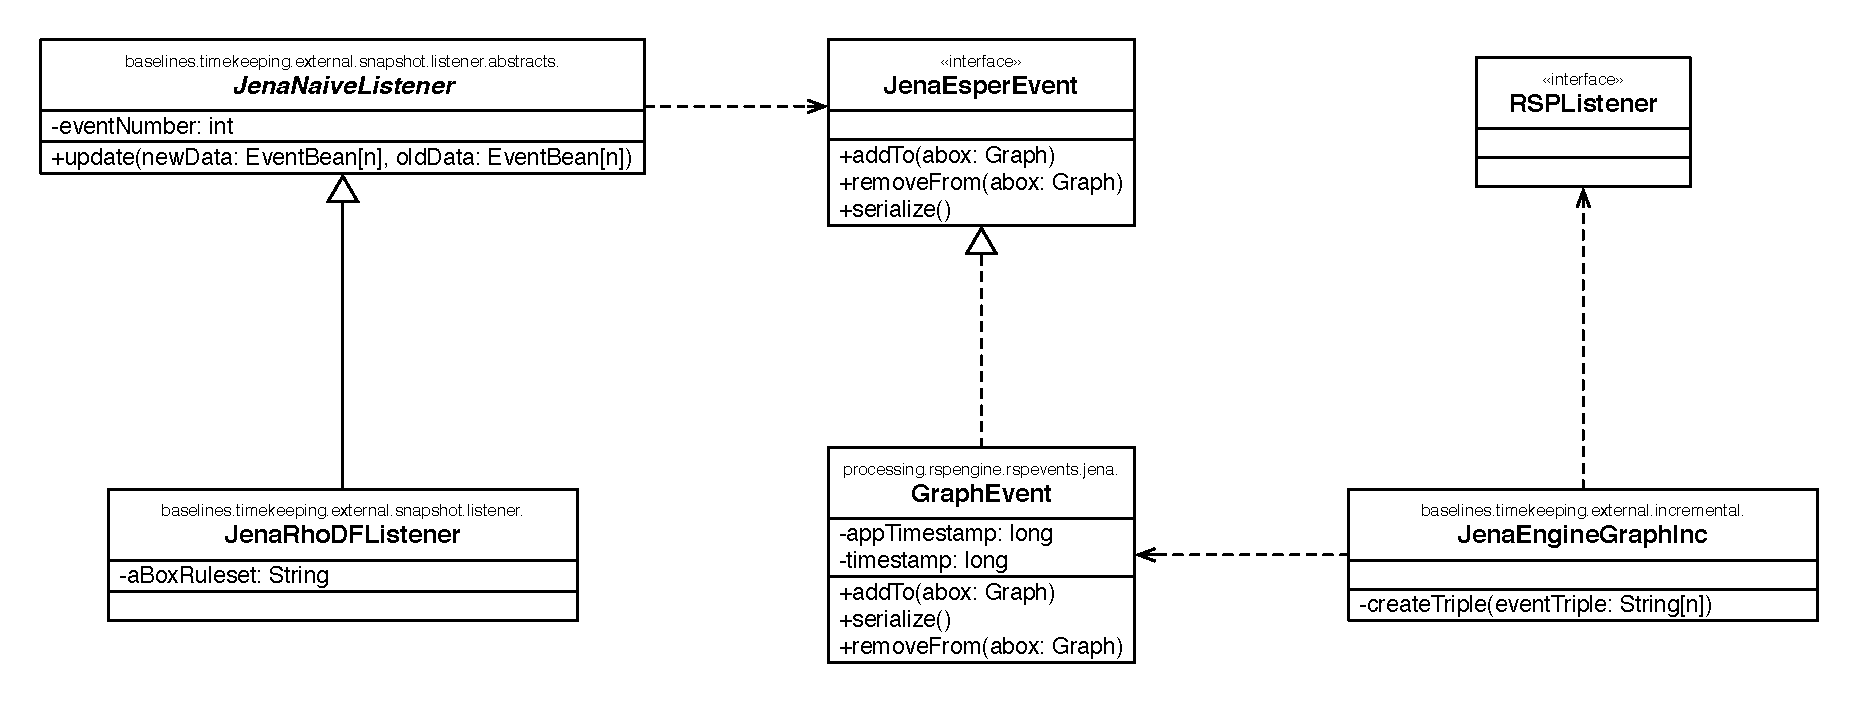
\includegraphics[width=\linewidth]{images/uml_baselines_rel_listener_event}
	\caption{RSPListener and events UML Schema} 
  	\label{fig:uml_baselines_rel_listener_event}
\end{figure}

This design allow the baselines to have a common design, sharing the majority of the code by splitting the different architectural elements. In this way we fulfil [R.16] which demands baseline Simplicity.


\section{Analyser}\label{sec:analyser-impl}

%R.9 allow qualitative analysis trough tools for result visualization



